\chapter{Theory}
\label{chap:Theory}
%This section documents the hardware of the Game Boy which must be emulated.

This section aims to describe the various components used in the Game Boy. This is needed to then be able to understand how to properly emulate the function of those components.

\section{The Central Processing Unit}
The Central Processing Unit (CPU) used in the Game Boy is a Sharp LR35902 \cite{pandoscspecifications} \cite{gameboyhistory} which is designed specifically for the Game Boy. The chip is heavily inspired by the Zilog Z80 \cite{Z80} and the Intel 8080 \cite{Intel8080}. While the CPU itself has a clock frequency of 4 MHz \cite{pandoscspecifications}, one can consider it having an actual clock speed of 1 MHz. 
This is due to the fact that the CPU is bound by the speed of the memory \cite{GBTClockSpeed} (the rate the RAM can provide data to the CPU) which has a clock speed of 1 MHz, see slide 149 of  \cite{ultimateGBtalkSlides}. 
%see slide 149
%In addition to this, the CPU is most probably following the fetch-decode-execute cycle, making a machine cycle equal to that of four clock cycles.
Furthermore, the CPU has a 16-bit address bus \cite{pandocsmemorymap} and an 8-bit arithmetic logic unit (ALU).
\subsection{Registers}
The CPU has six general purpose registers, B, C, D, E, H and L \cite{pandocsregistersandflags}. These are all 8 bits each, but can be used pairwise as three 16-bit registers, BC, DE and HL. There are also two additional 8-bit registers, A and F, which both have specific purposes. A is the accumulator register where all the arithmetic is done. The F register, despite being 8 bits, only uses 4 bits to store the value of the four flags of the ALU. These are the zero, negative, half-carry and carry flags \cite{pandocsregistersandflags}, abbreviated as Z, N, H and C respectively. Additionally, the CPU has a 16-bit program counter (PC) and stack pointer (SP).

\subsection{Instruction set}
In total the CPU supports 500 assembly instructions, of which 244 are 8-bit and 256 are 16-bit, see Figure \ref{fig:8bitOpCodes} for the 8-bit instructions. For the CPU to interpret the 16-bit operations, a certain prefix is used (\texttt{0xCB}) found in the 8-bit table allowing the CPU to interpret the following 8 bits as an instruction from the 16-bit table. The tables specify for each instruction which flags it affects, how many bytes it is encoded with and how many machine cycles it requires to execute. 
\\\\
\begin{figure}[H]
    \centering
    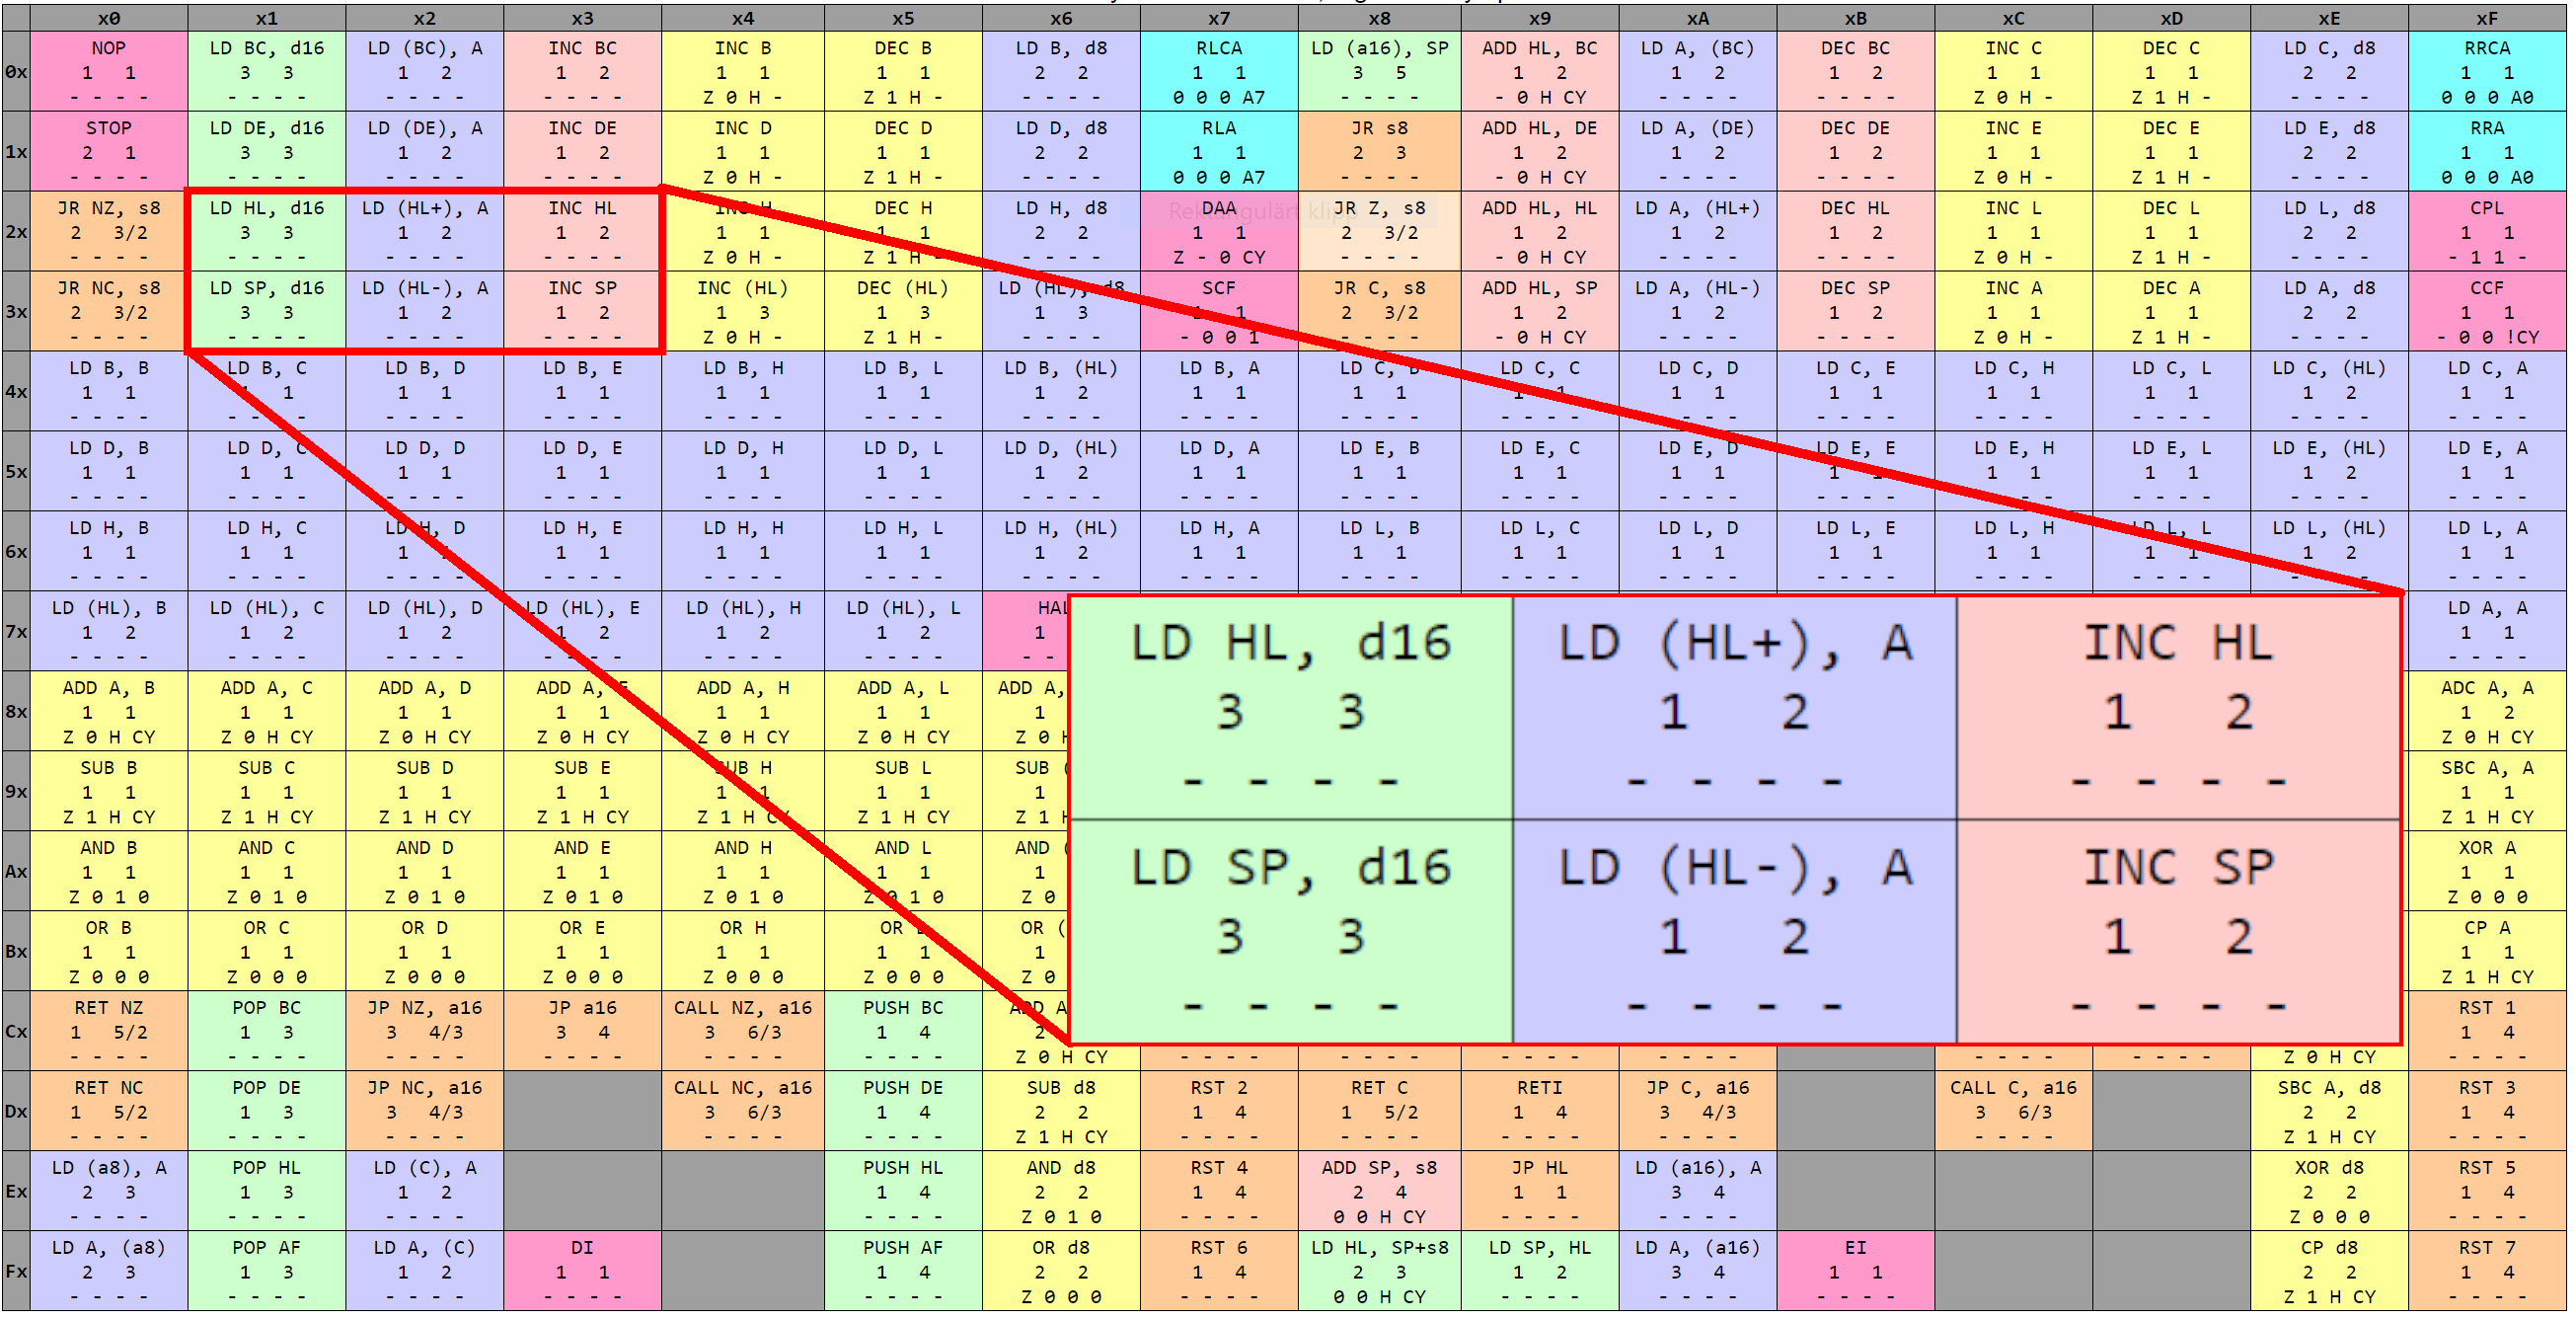
\includegraphics[width=\textwidth]{figures/8bitOpCodes.PNG}
    \caption{Displaying the 8-bit operation codes for the LR35902, highlighting six of the operation codes, showing their assembly instruction, number of bytes used, number of cycles to execute and what flags are affected. From \cite{OpCodes}. Modified with permission.}
    \label{fig:8bitOpCodes}
\end{figure}


%\begin{figure}[H]
%    \centering
%    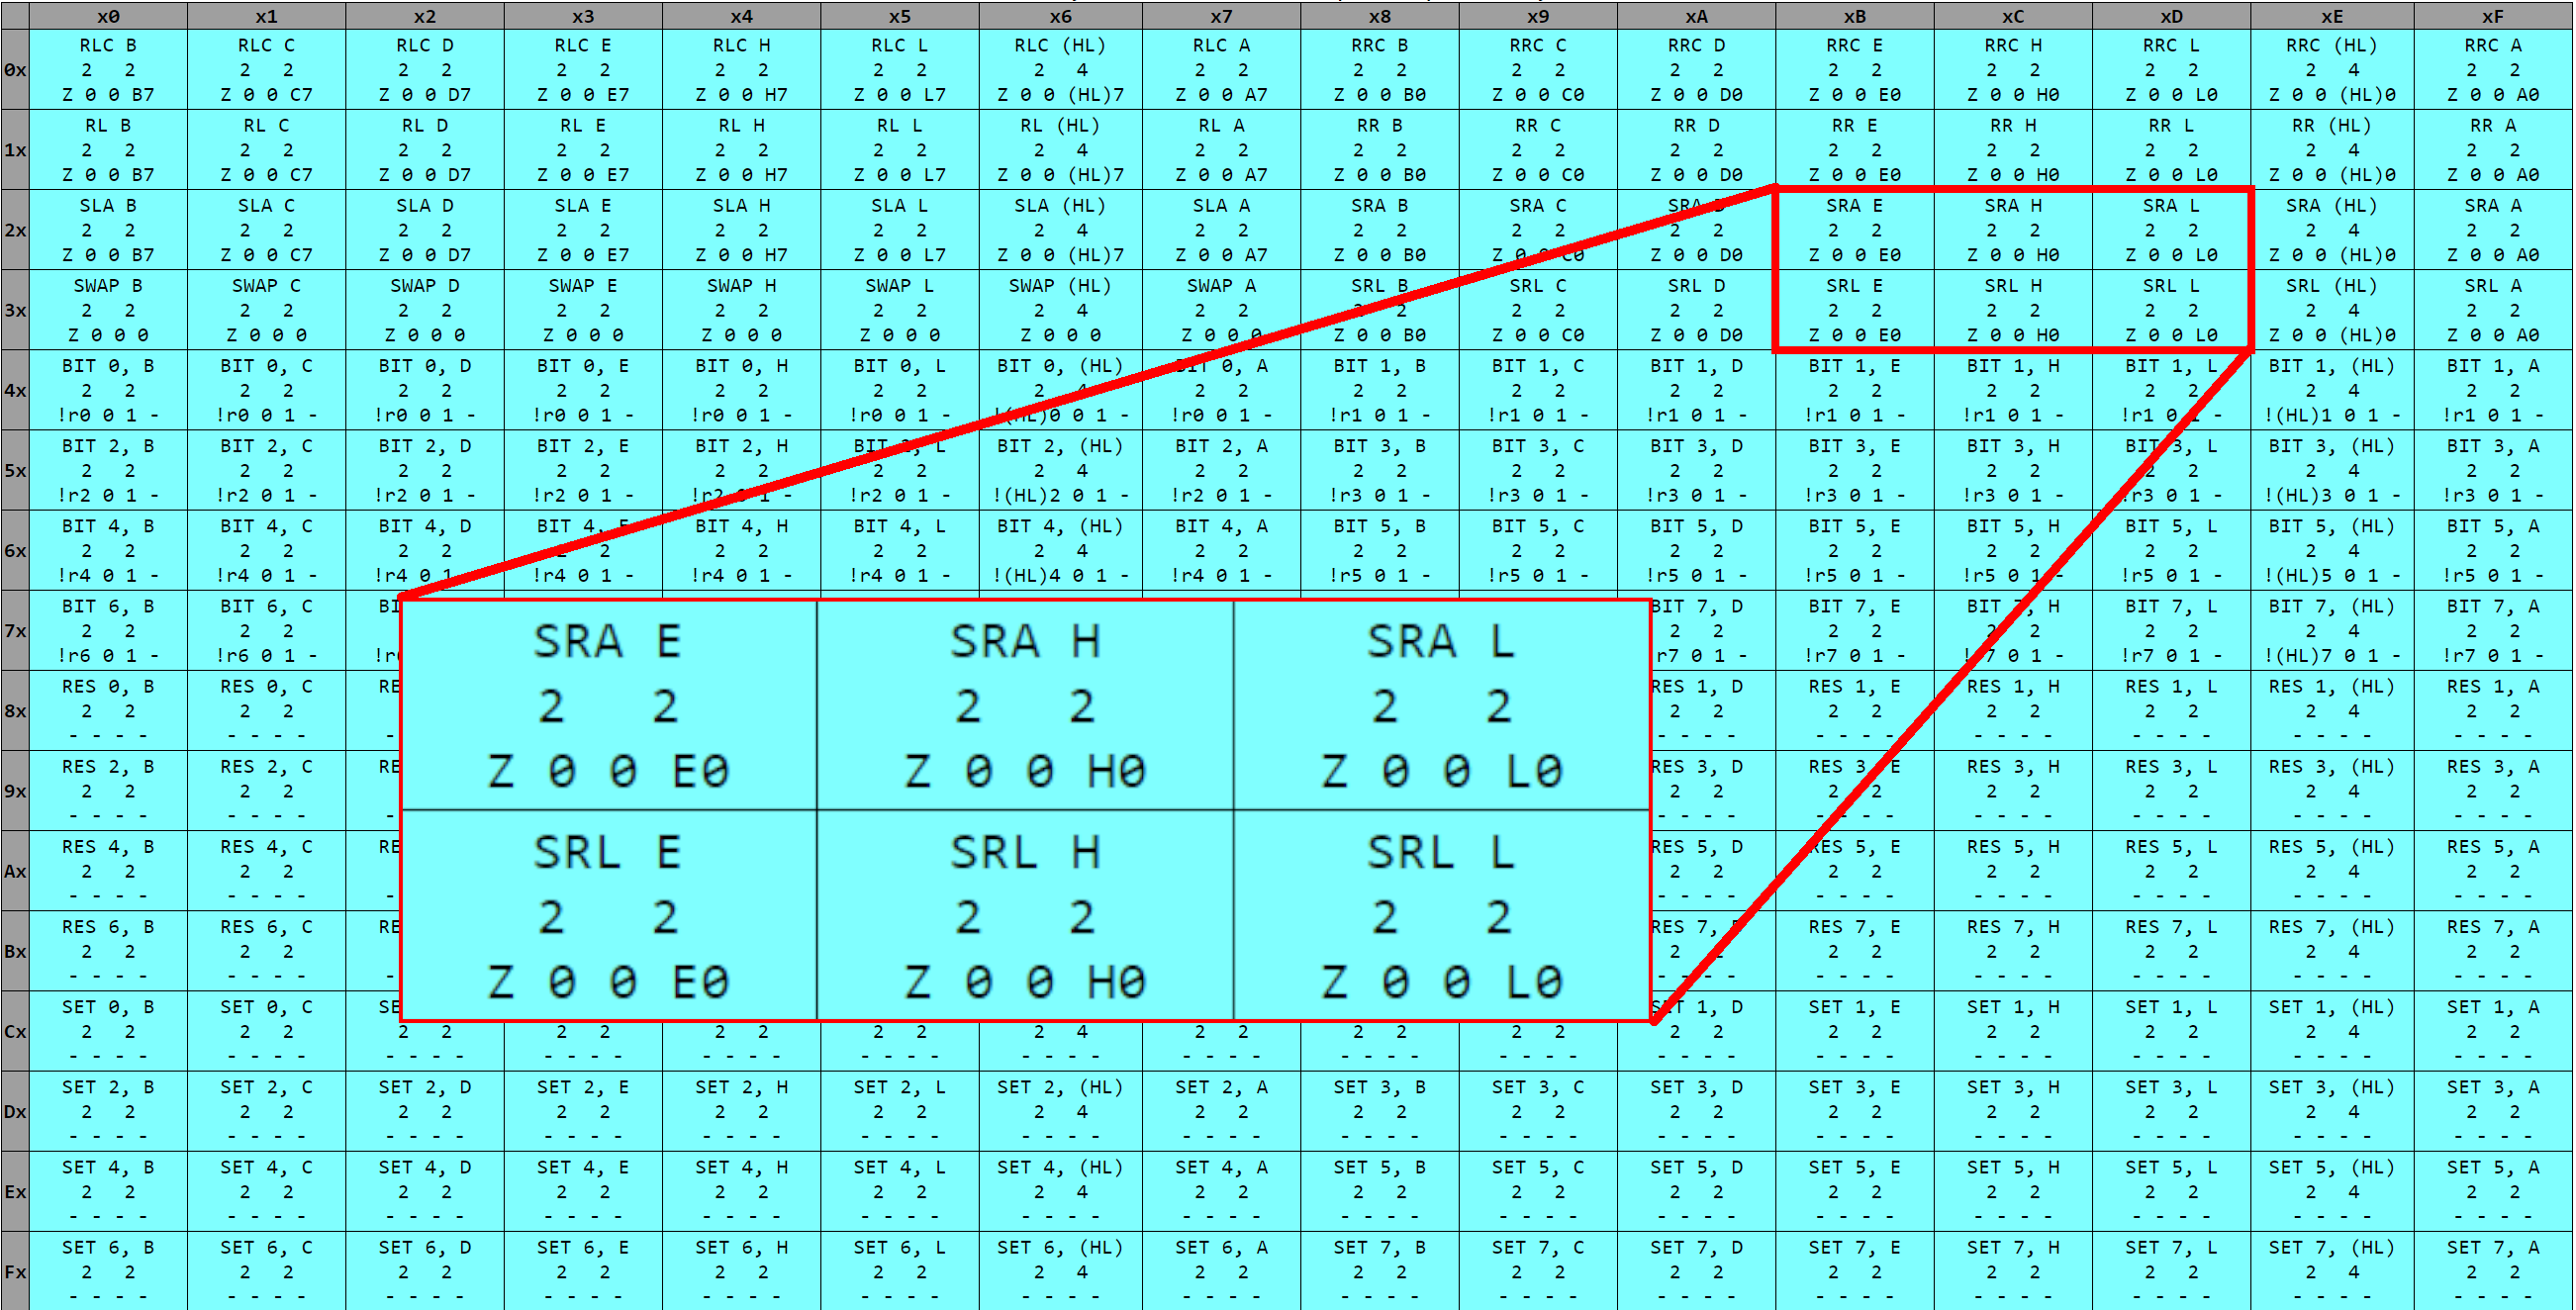
\includegraphics[width=\textwidth]{figures/16bitOpCodes.PNG}
%    \caption{Displaying the 16-bit operation codes for the %LR35902, highlighting six of the operation codes, showing their %assembly instruction, number of bytes used, number of cycles to %execute and what flags are affected. From \cite{OpCodes}. %Modified with permission.}
%    \label{fig:16bitOpCodes}
%\end{figure}
\subsection{Interrupts}
\label{sub}

Like many other CPUs, the Sharp LR35902 supports interrupts. Interrupts are used in order to break the regular flow of the CPU, forcing it to handle the interrupt before returning to what it was doing previously.
%The interrupts are handled by the CPU by continuously checking a number of bits and whether or not they are set.
Different interrupts have different pre-defined addresses where the respective interrupt routines are stored \cite{pandocsinterrupts}. When an interrupt occurs, the CPU executes the interrupt routine, and then continues execution from the address that was current when the interrupt occurred. The existing interrupts and their functionalities are the following \cite{pandocsinterrupts}:
\\
\begin{itemize}
    \item V-blank - An interrupt sent from the PPU when it has created a whole frame and wants to draw it, for more information see Section \ref{sec:PPU}.
    \item LCD STAT - A customisable interrupt regarding various conditions of the PPU. An interrupt is generated any time the PPU goes from not meeting any condition to meeting at least one condition. Which conditions are used is determined by the STAT register of the PPU, for more information, see Section \ref{sec:PPU_Registers}
    \item Timer - Sends an interrupt request when a set timer has run out, for more information see Section \ref{sec:Timer}.
    \item Serial - The serial transfer interrupt which handles the communication between two Game Boys when they are connected through the serial port. This is not implemented, as is explained in Section \ref{sec:Delimitations}.
    \item Joypad - An interrupt which handles the input from the joypad, for more information see Section \ref{sec:Joypad}.
    \\
\end{itemize}

The interrupts are implemented by having three different types of flag registers \cite{pandocsinterrupts}:
\begin{itemize}
    \item IME - Interrupt Master Enable. This flag enables and disables all other interrupt flags. Can only be manipulated through specific instructions.
    \item IE - Interrupt Enable. Enables or disables a specific flag. Consists of five bits, one for each type of interrupt. Manipulated through memory, located at \texttt{0xFFFF}.
    \item IF - Interrupt Flag. Shows that an interrupt has been requested. This is the flag which is set when an interrupt is raised. The register consists of five bits, one for each type of interrupt. Manipulated through memory, located at \texttt{0xFF0F}.
    \\
\end{itemize}
If IME is disabled, IE and IF can still be altered, but they are not acted upon until IME is enabled once again. For an interrupt to occur and be handled by the CPU three things therefore need to happen: both the IME flag and a specific IE flag must be enabled, and the corresponding IF flag must be triggered \cite{pandocsinterrupts}. 
\\\\
\newpage
\section{Memory and I/O devices}
\label{sec:MMUTheory}
The CPU needs to access memory and communicate with peripheral devices. To achieve this the Game Boy uses a 16-bit address bus and an 8-bit data bus \cite{TCAGBD}. The memory and different peripheral devices are mapped to specific memory addresses visualised in Figure \ref{fig:memory-map}.

%\begin{figure}[H]
%    \centering
%    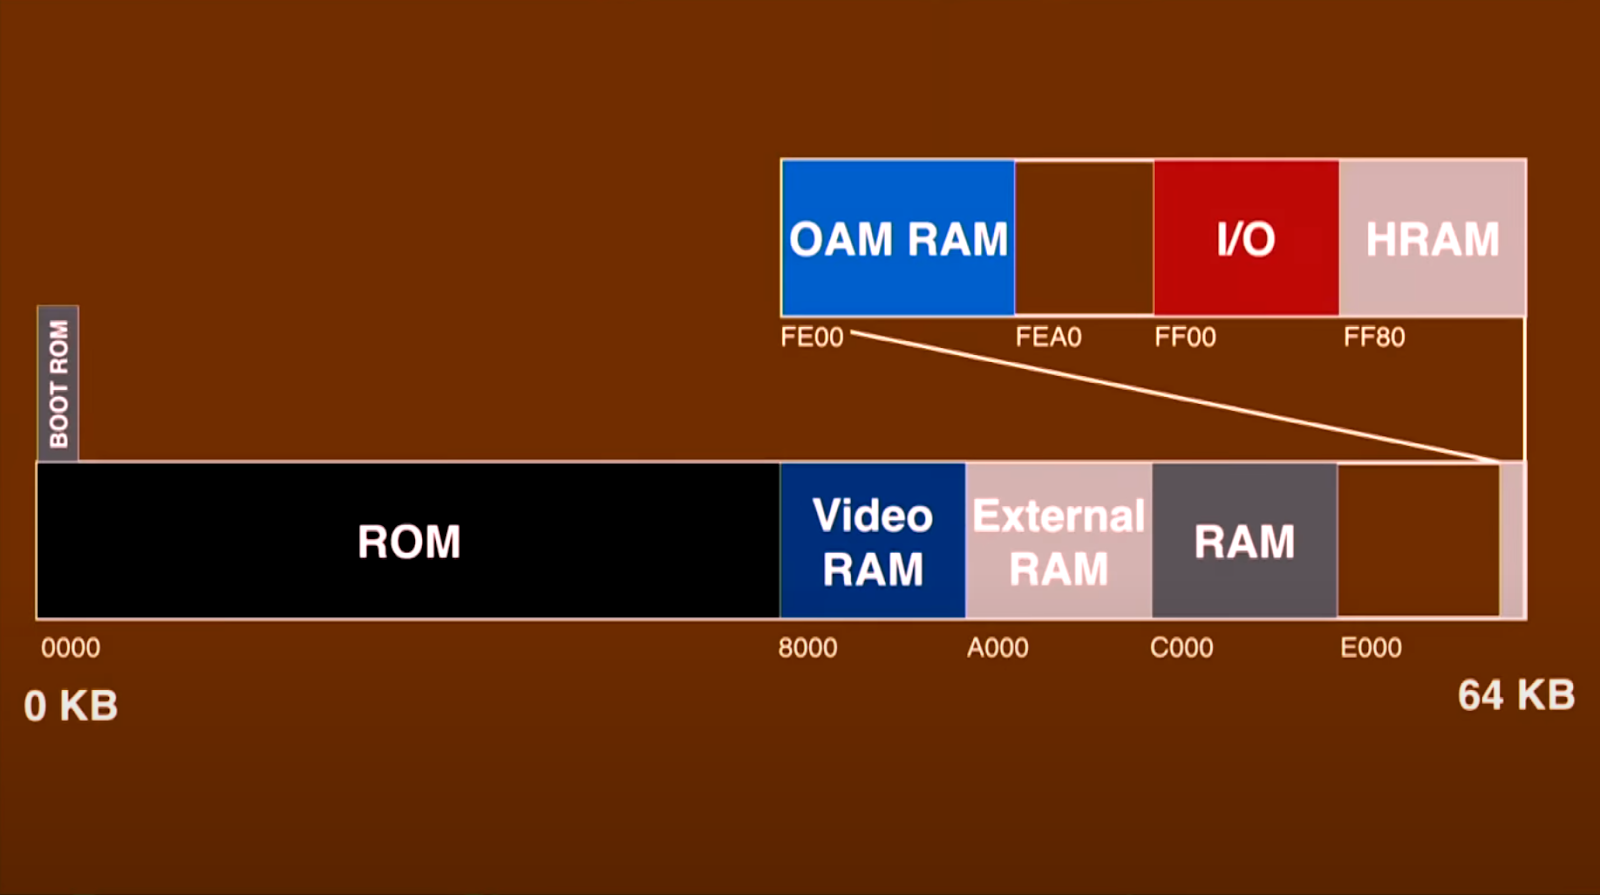
\includegraphics[scale=0.25]{figures/Memory.png}
%    \caption{Visual representation of how the address space is divided in the Game Boy \cite{GBTMem}.}
%    \label{fig:memory-map}
%\end{figure}

\begin{figure}[H]
    \centering
    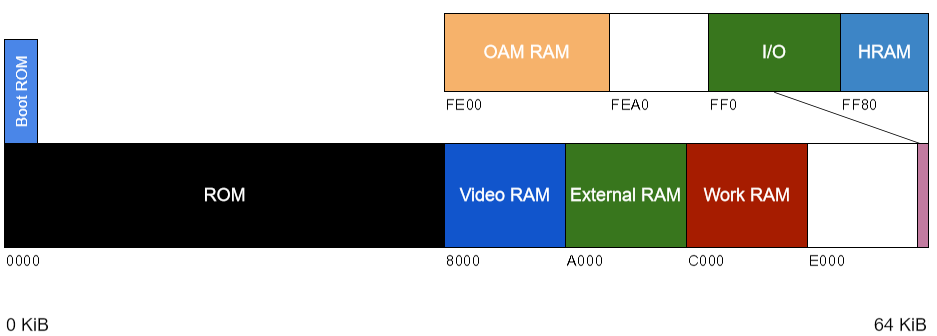
\includegraphics[width=\textwidth]{figures/Memory Map.PNG}
    \caption{Visual representation of how the address space is divided in the Game Boy. From \cite{ultimateGBtalkSlides}. Adapted with permission.}
    \label{fig:memory-map}
\end{figure}
In the Game Boy's 64 KiB address space, different address ranges are used for different purposes. Below is a description of how this is handled. Note that the I/O devices are controlled through manipulating address space and that the more complex I/O devices, the PPU and APU, are described in Section \ref{sec:PPU} and Section \ref{sec:APU} respectively.

\subsection{Boot ROM}
\textbf{Address: \texttt{0x00} - \texttt{0xFF}}

The boot ROM is a 256 byte ROM located on the DMG-CPU and contains the code that is executed when the Game Boy is powered on \cite{BootRom}. The purpose of the boot ROM is to initialise the different hardware units and prepare the Game Boy to execute game code \cite{bootstraptechopedia}. The official boot ROM used on the Game Boy does this while scrolling down the Nintendo logotype. The use of copyrighted material on the boot ROM has legal implications which is further discussed in Section \ref{sec:Ethics}.
In practice the boot ROM is only accessible a short time when the Game Boy is powered on due to the fact that it disables itself after it has been run. 
Disabling the boot ROM is done by storing a non-zero value at memory address \texttt{0xFF50} and will map the addresses to the ROM instead, see the overlap in Figure \ref{fig:memory-map}.
\newpage
\subsection{ROM}
\textbf{Address: \texttt{0x0000} - \texttt{0x7FFF}}
\\
The ROM located in the Game Boy's memory map is the area where the interactions with data from the inserted game ROMs happen \cite{pandocsmemorymap}. 
Although the allocated size for the ROM on the Game Boy is only 32 KiB, the ROMs it supports can be much larger. This is possible through the use of bank switching using a Memory Bank Controller (MBC) \cite{pandocsexternalmemoryandhardware}, located in the Game Pak ROM, see Section \ref{sec:MBC} for more information.

\subsection{Video RAM}
\textbf{Address: \texttt{0x8000} - \texttt{0x9FFF}}
\\
The Video RAM (VRAM) is an 8 KiB RAM \cite{pandocsmemorymap} that is accessible by both the CPU and PPU. 
It it used by the CPU to store data which the PPU uses for drawing. 
While the PPU is drawing, it is reading from the VRAM and the CPU is therefore not allowed access. 
For more information regarding how the VRAM is used, see Section \ref{sec:PPU}.


\subsection{External RAM}
\textbf{Address: \texttt{0xA000} - \texttt{0xBFFF}}
\\
The external RAM (XRAM) is an optional memory that is located on some of the game cartridges. Its size varies from game to game and can, if desired, also make use of bank switching (see Section \ref{sec:MBC}). The XRAM is often used for saving progress and high score tables \cite{pandocsmemorymap}. This is done by powering the XRAM with a small battery inside the game cartridge to make sure the data is conserved between different gaming sessions. 
\subsection{WRAM}
\textbf{Address: \texttt{0xC000} - \texttt{0xDFFF}}
\\
The Work RAM (WRAM) is the main memory of the system which is used by the CPU to store any data the game uses while running. The WRAM is located on the DMG-CPU and has a size of 8 KiB \cite{pandocsmemorymap}.


\subsection{OAM RAM}
\textbf{Address: \texttt{0xFE00} - \texttt{0xFE9F}}
\\
The Object Attribute Map (OAM) is the area where sprite data is stored. The OAM is divided into 40 blocks of four bytes each with each block corresponding to a sprite. Both the PPU and CPU have direct access to this memory area. While the PPU is rendering scanlines, the CPU has limited access to this area \cite{pandocsoam}. The CPU can also transfer data into the OAM through the use of Direct Memory Access (DMA) transfers, this process is described in detail in Section \ref{sec:DMA_transfer}.

%There is another way for the CPU to transfer data into OAM: Direct Memory Access (DMA) transfers. This process is described in detail in section \ref{sec:DMA_transfer}.



%\subsection{I/O devices}
%\textbf{Address: 0xFF00 - 0xFF7F}

%The I/O devices are controlled through reading and writing to their control and status registers.
%The more complex I/O devices, the PPU and APU are describes in their own chapters \ref{sec:PPU} and \ref{sec:APU} respectively. In this chapter the Joypad and the Timer will be described.
\subsection{Joypad}
\label{sec:Joypad}
%\subsubsection{Joypad}
\textbf{Address: \texttt{0xFF00}}
\\
The Joypad is the device that connects the user's input with the system. 
There are eight buttons on the Game Boy, four directional buttons: up, down, left and right, and four action buttons: A, B, Start and Select.
The buttons have two states, pressed or not pressed. 
These states of the buttons are stored at address \texttt{0xFF00} as a 2x4 matrix \cite{pandocsjoypad}.
\\\\
By writing specific values to bit 4 and 5 either the action buttons or directional buttons will be selected.
When selecting either the action or direction buttons bit 0-3 will correspond to the selected buttons \cite{pandocsjoypad}. See Table \ref{tab:joypad}.


\begin{table}[H]
    \begin{center}

\begin{BVerbatim}
Bit 7 - Not used
Bit 6 - Not used
Bit 5 - Select Action buttons    (0=Select)
Bit 4 - Select Direction buttons (0=Select)
Bit 3 - Input: Down  or Start    (0=Pressed) (Read Only)
Bit 2 - Input: Up    or Select   (0=Pressed) (Read Only)
Bit 1 - Input: Left  or B        (0=Pressed) (Read Only)
Bit 0 - Input: Right or A        (0=Pressed) (Read Only)
\end{BVerbatim}

    \caption{Layout of the button states located in memory address \texttt{0xFF00}. From \cite{pandocsjoypad}. Adapted with permission.}
    \label{tab:joypad}
    \end{center}
\end{table}

When a button is pressed, an interrupt is raised, but only if the pressed button is a button that is selected by bit 4 and 5 (either an action or a directional button) \cite{pandocsjoypad}. Regarding how to actually handle the joypad input, it is up to the developer to either poll the $2 \times 4$ -matrix or by using the interrupts.

\subsection{Timer}
\label{sec:Timer}
%\subsubsection{Timer}

\textbf{Address: \texttt{0xFF04} - \texttt{0xFF07}}

The Game Boy has a built-in timer which can be used to perform time sensitive tasks. 
It is used and controlled by reading and writing to the following registers \cite{pandocstimer}:
\\\\
\textbf{Divider Register - DIV}
\\
\textbf{Address: \texttt{0xFF04}}
\\
The DIV register is a counter that always increments at a rate of 16384Hz. 
When writing any value to the address the counter resets to 0 \cite{pandocstimer}.
\\\\
\newpage
\textbf{Timer counter - TIMA}
\\
\textbf{Address: \texttt{0xFF05}}
\\
This is another counting register, it increments at the rate that is specified in the TAC register. 
When the counter value is 0xFF and overflows it is reset to the value in TMA as the new counter value.
When the counter overflows the ``Timer''-interrupt is raised \cite{pandocstimer}.
Writing to this register simply changes the counter to the written value.
\\\\
\textbf{Timer Modulo - TMA}
\\
\textbf{Address: \texttt{0xFF06}}
\\
This register holds the timer modulo value.
This value is loaded into the TIMA register when the TIMA counter overflows \cite{pandocstimer}.
It can be used to further modify the chosen clock speed chosen in the TAC register.
\\\\
\textbf{Timer Control - TAC}
\\
\textbf{Address: \texttt{0xFF07}}
\\
This register is used to control the timer.
By writing to this register the timer can be enabled or disabled. The rate at which the TIMA register will increment can also be controlled by writing to this register \cite{pandocstimer}. 
\\\\
As shown in Table \ref{tab:timer_tac}, bit 2 enables or disables the timer. 
Notice that disabling the timer does not stop the DIV counter.
Bits 0 and 1 are used to select one out of four possible clock speeds; 4069 Hz, 262144 Hz, 65536 Hz or 16384 Hz \cite{pandocstimer}. 

\begin{table}[H]
    \begin{center}

\begin{BVerbatim}
Bit  2   - Timer Enable
Bits 1-0 - Input Clock Select
           00: CPU Clock / 1024 (4096 Hz)
           01: CPU Clock / 16   (262144 Hz)
           10: CPU Clock / 64   (65536 Hz)
           11: CPU Clock / 256  (16384 Hz)
\end{BVerbatim}

    \caption{Layout of the each bit in the timer control register located at address \texttt{0xFF07}. From \cite{pandocstimer}. Modified with permission.}
    \label{tab:timer_tac}
    \end{center}
\end{table}

\subsection{HRAM}
\textbf{Address: \texttt{0xFF80} - \texttt{0xFFFE}}

The high RAM or HRAM is very much like the WRAM although it is much smaller and faster to access. 
It is faster because of a special instruction that assumes that the highest byte in the address is \texttt{0xFF} and therefore saves time decoding the instruction \cite{OpCodes}. 
During a DMA-transfer (see Section \ref{sec:DMA_transfer}) the CPU is limited to use only this memory.
The size of the HRAM is 126 bytes \cite{pandocsmemorymap}. 
\newpage
\subsection{Memory Bank Controllers}
\label{sec:MBC}
As previously mentioned, the Game Boy uses a 16-bit address bus, which in turn limits the memory addresses available for the game ROM and external RAM. 
To bypass this limitation many game cartridges make use of a memory bank controller (MBC).
The MBC is used to map different sections of a memory, called memory banks, to one specific address range, this method is called bank switching.
It works as follows: reading from addresses \texttt{0x0000} to \texttt{0x7FFF} returns a byte stored on the ROM as expected, but writing to those same addresses will instead change the MBC's control registers, this is further described below and in Figure \ref{fig:MBC3}. 
These control registers control what memory bank is to be used for both the game ROM and the external RAM (if any).
\\\\
There are different versions of MBCs which all support various arrangements of additional hardware. 
Examples of such hardware are external RAM with or without a battery powering said RAM and in some cases also a timer \cite{GBWikiMBC}. For example, MBC3 supports up to 2 MiB of ROM and/or 64 KiB of RAM, and Real Time Clock (RTC) with battery \cite{GBWikiMBC}.

\begin{figure}[H]
    \centering
    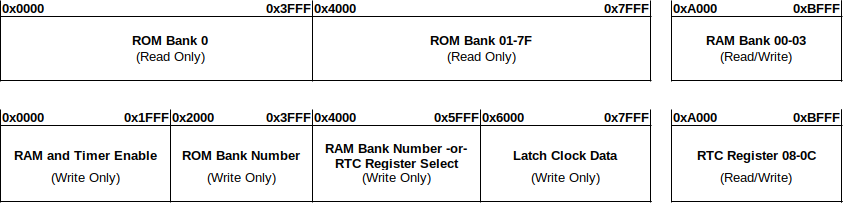
\includegraphics[scale=0.5]{figures/MMU/MBC3_figure_no_padding.png}
    \caption{Memory map of MBC3. While all MBCs do not necessarily contain the same features, most follow a similar structure \cite{GBWikiMBC}.}
    \label{fig:MBC3}
\end{figure}

The following is a description of the structure and functionality of MBC3, shown in Figure \ref{fig:MBC3} \cite{GBWikiMBC}:
\\\\
\textbf{ROM Bank 0 }
\\
Contains the first 16 KiB of the ROM.
\\\\
\textbf{ROM Bank 0x01-0x7F}
\\
This part of the memory is used for bank switching. There are at most 127 available memory banks each with a size of 16 KiB, resulting in a total ROM size of $128 \times 16$ KiB = 2 MiB, including ROM bank 0.
\\\\
\textbf{RAM and Timer Enable}
\\
Writing specific values to this address will enable reading and writing to XRAM or RTC registers depending on which is currently active.
\\\\
\textbf{ROM Bank Number}
\\
Writing to this address controls which ROM bank is in use.
\\\\
\textbf{RAM Bank Number/RTC Register Select}
\\
Writing to this area maps the corresponding XRAM bank or RTC register into the memory of \texttt{0xA000}-\texttt{0xBFFF}. 
\\\\
\textbf{RAM Bank 0x00-0x03 or RTC Register 0x08-0x0C}
\\
Depending on the current \textbf{Bank Number/RTC Register selection}, this memory space is used to either access an 8 KiB external RAM Bank, or a single RTC Register, see Table \ref{tab:rtc_registers}.
\\\\
\textbf{Latch Clock Data}
\\
If writing first 0x00, and then 0x01 to this register, the current time becomes latched into the RTC register. This means that the current time can be read from the register while the RTC continues to tick. Additionally the RTC needs a quartz oscillator as well as an external battery to work while the Game Boy is turned off. 
\\\\
\begin{table}[H]
    \begin{center}

\begin{BVerbatim}
0x8  RTC S   Seconds   0-59 (0x00-0x3B)
0x9  RTC M   Minutes   0-59 (0x00-0x3B)
0xA  RTC H   Hours     0-23 (0x00-0x17)
0xB  RTC DL  Lower 8 bits of Day Counter (0x00-0xFF)
0xC  RTC DH  Upper 1 bit of Day Counter, Carry Bit, Halt Flag
      Bit 0  Most significant bit of Day Counter (Bit 8)
      Bit 6  Halt (0=Active, 1=Stop Timer)
      Bit 7  Day Counter Carry Bit (1=Counter Overflow)
\end{BVerbatim}

    \caption{List of the different RTC registers and its contents. From \cite{pandocsmbc}. Adapted with permission.}
    \label{tab:rtc_registers}
    \end{center}
\end{table}


%\end{comment}

\newpage
\section{The Pixel Processing Unit}
\label{sec:PPU}

The purpose of the Pixel Processing Unit (PPU) is to interpret the data residing in VRAM and compose it into a picture which can then be printed on the LCD. The CPU can communicate with the PPU either by loading data into the VRAM or by reading from or writing to a number of hardware registers, most notably the LCD control and status registers. The PPU, on the other hand, uses interrupts to communicate with the CPU \cite{pandocsVideo}.

\subsection{Composing the frame}
\label{sec:PPU_image}

The frame is composed of three layers: Background, Window and Sprites, rendered in that order. These layers are in turn composed of tiles, 8x8 bitmaps of colour indices, which are stored in VRAM. When rendering the picture, these indices map to one of the four colours using palette tables, which in the original Game Boy was four shades of grey over a green background \cite{gameboyarchitecture}. The following is a description of the components used to form the frame.\\
\\
\textbf{Tiles} - 
As previously mentioned, the tiles are 8x8 bitmaps stored in RAM, 16 bytes per tile. This is because each row of a tile is formed by combining the bits of two bytes. The bytes are organised in two memory regions called \textit{Tile sets}; one ranging from \texttt{0x8000} to \texttt{0x9000} and one ranging from \texttt{0x8800} to \texttt{0x9800}, see Figure \ref{fig:ppu_tile_set}. These two tile sets overlap and which one to use is determined by a bit in the LCD Control register (LCDC). The first of the two uses unsigned addressing for tile IDs, while the second one uses signed addressing. \cite{gameboyarchitecture}.
\newpage
\begin{figure}[H]
    \centering
    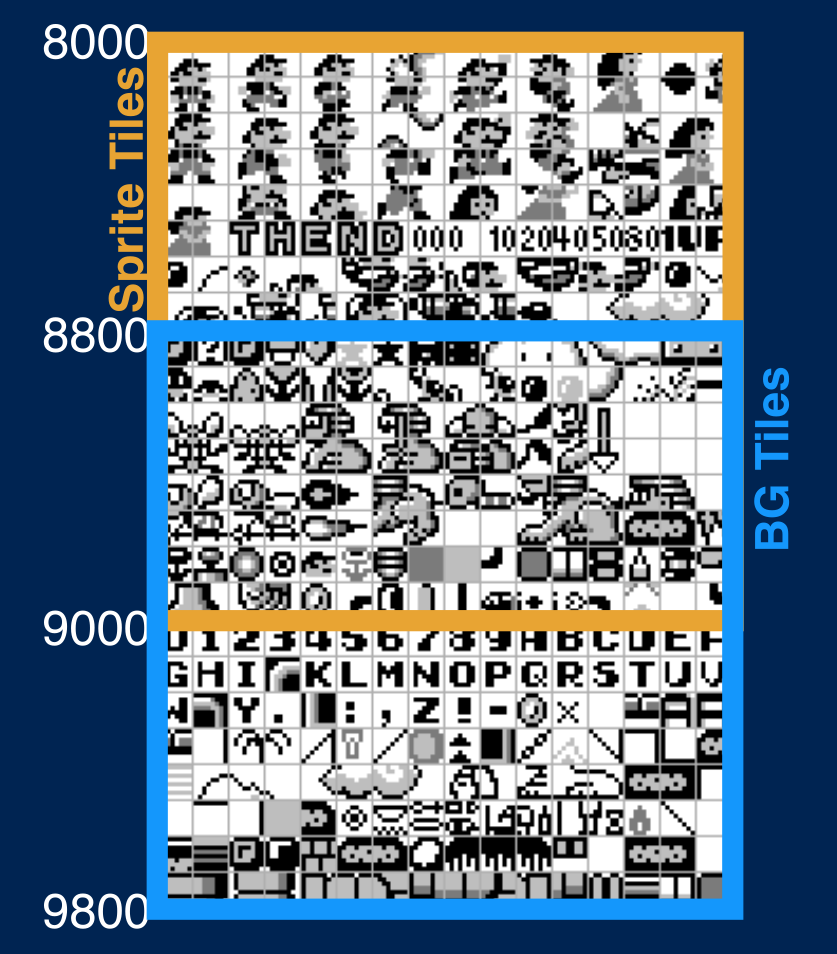
\includegraphics[width=0.8\linewidth]{figures/PPU/PPU_tile_sets_divided.png}
    \caption{The two tile sets. Sprites may only use tiles from the tile set ranging from \texttt{0x8000} to \texttt{0x9000} while the background and window can use any of the two sets. From \cite{ultimateGBtalkSlides}. Used with permission.}
    \label{fig:ppu_tile_set}
\end{figure}
%Slide 434
\textbf{Background} - 
The background is defined by a map of 32x32 tile IDs. Since a tile is 8x8 pixels, this results in a map of 256x256 pixels; however, the Game Boy's display is only 160x144 pixels. The result of this is that only part of the background is being displayed at any given time, as shown in Figure \ref{fig:ppu_viewport}. Which part of the map to display is determined by the two hardware registers, SCX and SCY, which specify which pixel should appear in the top left corner of the display. If the edge of the map is reached, the map loops around and continues at the opposite side. There are also two maps available at any given time, which one is being used is determined by a bit in the LCDC \cite{pandocsVideo}.\\
\\
\begin{figure}[H]
    \centering
    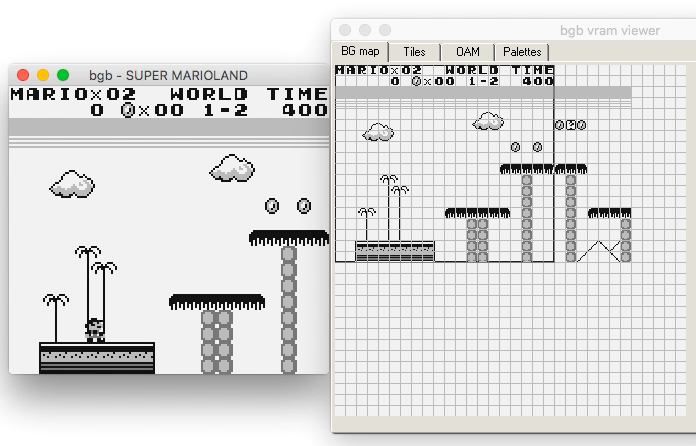
\includegraphics[width=\linewidth]{figures/PPU/PPU_viewport.png}
    \caption{What is shown on the LCD in relation to the background map. From \cite{ultimateGBtalkSlides}. Used with permission.}
    \label{fig:ppu_viewport}
\end{figure}
%Slide 320
\textbf{Window} - 
The window is drawn on top of the background. Just like the background, it consists of a map of tiles; however, this map is only 20x18 tiles, just covering the entire screen and, unlike the background, does not loop around. This layer can be used to display information that should not scroll with the rest of the background, such as a GUI \cite{pandocsVideo}.\\
\\
\textbf{Sprites} - 
Sprites are objects that can move around on the screen freely. They consist of one or two tiles, depending on a bit in the LCDC register. As opposed to the tiles in the background and window layers, sprites can have transparent pixels, meaning that the background and window are still visible through said pixels. Sprites only consist of tiles from the tile set ranging from \texttt{0x8000} to \texttt{0x9000}, as shown in Figure \ref{fig:ppu_tile_set} \cite{pandocsVideo}.\\
\\
Sprite data is stored in a memory region called the Object Access Map(OAM). Each sprite takes up four bytes of memory. These bytes store the sprites' x and y coordinates, the sprites' tile IDs and a set of flags. The flags describe which of two object palettes the sprite uses, whether the sprite is flipped horizontally or vertically, and lastly whether the sprite should be drawn in front of or ``behind'' the background. Drawing a sprite ``behind'' the background results in background and window pixels with colour indices 1-3 being drawn in front of the sprite, though the sprite is still drawn in front of pixels with colour index 0 \cite{pandocsVideo}.

\subsection{The modes}
\label{sec:PPU_Modes}
At any given time, the PPU is in one of four modes: horizontal blanking, vertical blanking, OAM search or drawing \cite{pandocsVideo}.

\begin{figure}[H]
    \centering
    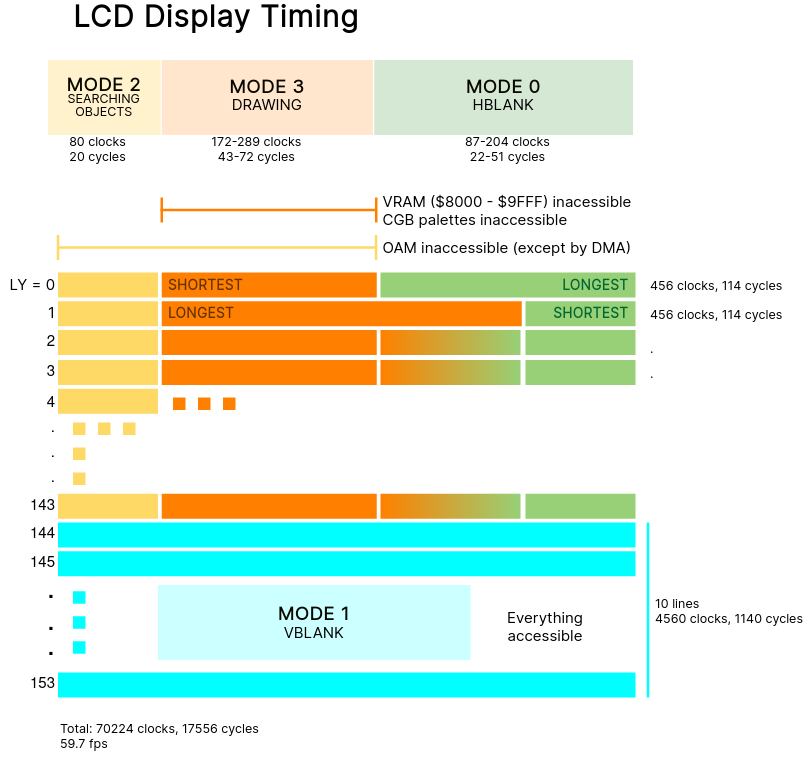
\includegraphics[scale=0.5]{figures/PPU/Mode_diagram.png}
    \caption{The various PPU modes and their durations. From \cite{pandocs}. Public Domain.}
    \label{fig:PPU_timing}
\end{figure}

Depending on which mode the PPU is in, there are limits on whether the CPU has direct access to VRAM and OAM. When the CPU does not have access to one of these regions, any write to that region will be ignored and any read will return 0xFF. The PPU changes modes according to Figure \ref{fig:PPU_timing} \cite{pandocsVideo}. The four modes will now be described in further detail.\\
\\
\textbf{Horizontal blanking}
\\
The PPU enters a horizontal blank (H-blank) whenever it has finished drawing a line. During this period, the CPU can access VRAM and OAM freely. Depending on how long the PPU was in mode 3 before entering this mode, the length of the H-blank is adjusted so that the total time spent on OAM search, drawing and H-blanking for each line is exactly 114 cycles \cite{pandocsVideo}.\\
\\
\textbf{Vertical blanking}

The PPU enters a vertical blank (V-blank) whenever all 144 scanlines have been drawn to the screen. The V-blank is treated as ten blank lines and therefore lasts for 1140 cycles. During this time the CPU has free access to VRAM and OAM \cite{pandocsVideo}.\\
\\
\textbf{OAM search}

The PPU enters this mode before drawing each line. When in this mode, the PPU finds the first ten sprites in OAM that intersect the current scanline to prepare for the draw phase. During this time the CPU can access VRAM freely \cite{pandocsVideo}. \\
\\
\textbf{Drawing}

The PPU enters this mode after having finished OAM search. During this mode the PPU combines the background, window and sprites of the current row and draws the pixels to the LCD. The process is described in more detail in Section \ref{sec:PPU_Drawing}. During this time the CPU can access neither VRAM nor OAM \cite{pandocsVideo}. 

\subsection{The registers}
\label{sec:PPU_Registers}

The PPU contains a variety of hardware registers. These are described in this section, also noting whether they are used for reading or writing to. \\
\\
\textbf{LCD Control Register (R/W)}\\
The LCDC register is the main way for the CPU to control the operation of the PPU. It can be modified at any time and contains the following bits \cite{pandocsLCDC}:\\
\\
\begin{itemize}
    \item Bit 7 - LCD enable. If this bit is 0, the display is off.
    \item Bit 6 - Window tile map select. This bit determines which map should be used for the window layer.
    \item Bit 5 - Window enable. This bit determines whether the window layer should be drawn or not.
    \item Bit 4 - Tile set select. This bit determines which tile set should be used by the tile maps.
    \item Bit 3 - Background tile map select. This bit determines which map should be used for the background layer.
    \item Bit 2 - Object size. This bit determines whether sprites consist of one or two tiles.
    \item Bit 1 - Object enable. This bit determines whether sprites should be drawn or not.
    \item Bit 0 - Background and window enable. This bit determines whether the background and window layers should be drawn or not.
\end{itemize}

\vspace{30pt}
\newpage
\textbf{LCD Status and Configuration Register (R/W)}\\
The STAT register represents the status of the PPU. It can also be used to create custom interrupts, depending on the status of the PPU. The STAT register contains the following bits \cite{pandocsSTAT}:\\
\\
\begin{itemize}
    \item Bit 6 - LYC interrupt enable. Enables interrupts when the current scanline equals the value of the LYC register.
    \item Bit 5 - OAM search interrupt enable. Enables interrupts when the PPU enters OAM search.
     \item Bit 4 - V-blank interrupt enable. Enables interrupts when the PPU enters a V-blank.
    \item Bit 3 - H-blank interrupt enable. Enables interrupts when the PPU enters an H-blank.
    \item Bit 2 - LYC=LY flag. Is set to 1 if the current scanline equals the value of the LYC register.
    \item Bit 1-0 - Mode flag. Represents the current mode of the PPU.
\end{itemize}

\vspace{30pt}

The PPU also has a variety of utility registers, described here \cite{pandocsVideo}:\\
\\
\begin{itemize}
    \item SCY and SCX (Scroll X \& Y) - Control background scrolling. Represents the coordinate on the background map that should be displayed in the top left corner of the display. (R/W)
    \item LY (Line Y) - Keeps track of the current scanline. (R)
    \item LYC (Line Y Compare) - Used in the STAT register to generate interrupts. (R/W)
    \item WY and WX (Window X \& Y) - Represents the coordinate on the display where the top left pixel of the window should be displayed. (R/W)
%    \item BGP (Background Palette) - The palette for the background. Maps the colour indices 0-3 to the colours white (0), light grey (1), dark grey (2) and black (3). (R/W)
    \item BGP (Background Palette) - The palette for the background. Maps the indices 0-3 to white (0), light grey (1), dark grey (2) or black (3). (R/W)
    \item OBP0 (Object Palette 0) - The first of two sprite palettes. Functions similarly to BGP except colour index 0 represents transparent pixels. (R/W)
    \item OBP1 (Object Palette 0) - The second of two sprite palettes. Functions exactly like OBP0. (R/W)
    \item DMA (Direct Memory Access) - Used for triggering a DMA transfer. More information can be found in Section \ref{sec:DMA_transfer}.  (R/W)
\end{itemize}
\newpage
\subsection{Drawing the image}
\label{sec:PPU_Drawing}
During mode 3 the PPU continuously transfers pixels to the LCD. This is done by loading tile data into two FIFO queues, one row of pixels at a time. One queue stores background  and window pixels and the other queue stores sprite pixels. The pixels are then popped from the queues and mixed depending on whether the sprite or the background should have priority \cite{pandocsDrawing}. This is also where the colour indices are mapped to colours using the palette tables. Depending on how many sprites are on the current scanline and whether the background is scrolled or not, the duration of mode 3 may be lengthened or shortened \cite{pandocsDrawing}. This results in mode 3 lasting between 43-72 cycles, as shown in Figure \ref{fig:PPU_timing}.

\subsection{Direct Memory Access transfer}
\label{sec:DMA_transfer}
As mentioned previously, the CPU can access OAM freely during H-blanks and V-blanks. There is however another way to update the OAM: through Direct Memory Access transfers (DMA transfers). A DMA transfer is triggered by writing a value between 0x00 and 0xDF to the DMA register \cite{pandocsdma}. This value is bit-shifted to the left eight times and is then used as the start address for the transfer, where the PPU copies the $40 \times 4 = 160$ following bytes into the OAM. During the transfer, which takes 160 cycles, the CPU can only access HRAM and no sprites are displayed. This process can be used no matter which mode the PPU is in, though there may be visual bugs if a transfer is started when the PPU is in mode 3 \cite{pandocsdma}.
\newpage
\section{The Audio Processing Unit }
\label{sec:APU}
The role of the Audio Processing Unit (APU) is to play audio. The Game Boy can play sound through four separate channels, each of which is an independently controllable source of sound \cite{pandocssound}. Each individual channel has a designated waveform assigned to it with each waveform defining what type of sound the respective channel plays. A waveform can be visually represented through a graph that shows change of amplitude over time. These waveforms sound drastically different to each other, which makes for a highly customisable sound experience even with only four channels available. The first two channels are only able to play pulse waves (see Figure \ref{fig:square_wave_forms}), the third channel has a programmable waveform, which enables some customisability for the game developer, and the fourth channel plays a pseudo-random waveform, producing noise \cite{AudioHardware}. For further information about how waveforms and sound in general works, see \cite{waveforms} and \cite{sinToSquare}.
%These channels differ between each other by what waveform they can play, i.e. the shape of the sound wave which is played. 
%There are three kinds of waveforms used by the Game Boy. The square wave, which is characterised by instantly changing between its maximum and minimum https://www.teachmeaudio.com/recording/sound-reproduction/waveshapes
%https://www.planetanalog.com/llc-power-conversion-explained-part-2-sine-wave-from-a-square-wave/
%https://soundbridge.io/what-are-waveforms-how-they-work/
%value and the other way around. The wave
%Of these four channels, there are two which only can play pulse waves (see Figure \ref{fig:square_wave_forms}), one which has a programmable waveform, where the game can decide exactly what sound to make, and one which only play pseudo-random waveform, also known as noise \cite{AudioHardware}. 

\subsection{The registers}
    The APU has a large number of registers for controlling the audio output for each channel. Settings such as volume and frequency can be changed by writing to the registers of each channel. The layout of these registers can be seen in Figure \ref{fig:apu_channel_registers}. The labels for each bit in Figure \ref{fig:apu_channel_registers} corresponds to a specific functionality described in Table \ref{tab:channel_reg_table}.

    \begin{figure}[H]
        \centering
        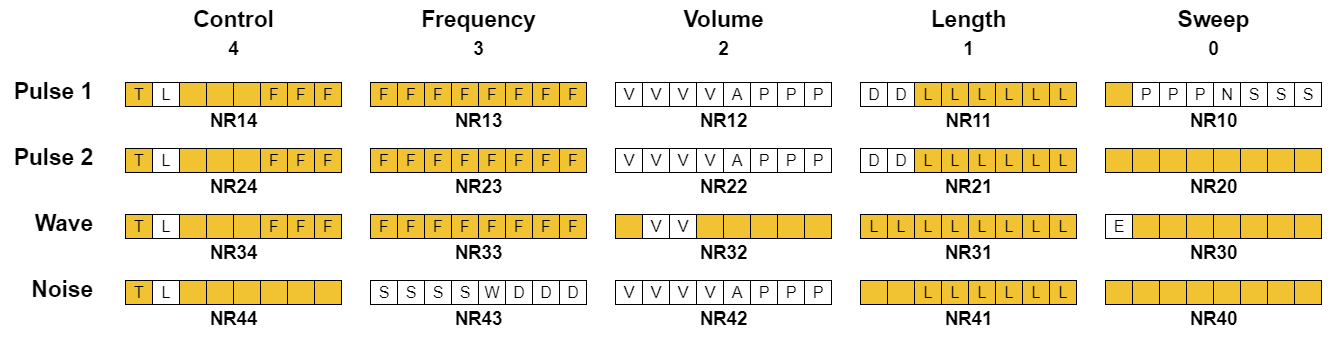
\includegraphics[width=\linewidth]{figures/APU/apu_channel_registers.png}
        \caption{The registers NR10-NR44, addresses \texttt{0xFF10}-\texttt{0xFF23}, for controlling audio channels. Bits coloured in yellow are write only and will always return 1 if read from \cite{AudioHardware}. From \cite{ultimateGBtalkSlides}. Adapted with permission. }
        \label{fig:apu_channel_registers}
    \end{figure}
    
    \begin{table}[h]
        \centering
        \begin{tabular}{|c|c|c|}
            \hline
            \textbf{Label} & \textbf{Name} & \textbf{Functionality} \\
            \hline
            T & Toggle & Turns the channel on or off \\
            \hline
            L (NRx4) & Length enable & \multirow{3}{*}{\shortstack{If the channel should be\\turned off after a short\\period of time}} \\
            & & \\
            & & \\
            \hline
            F & Frequency & \multirow{4}{*}{\shortstack{How long to play\\each audio sample}} \\
            \cline{1-2}
            S, W, D (NR43) & Clock Shift &  \\
            &  LFSR mode & \\
            & Divisor code & \\
            \hline
            V, A, P (Not NR32) & Volume & \multirow{3}{*}{\shortstack{Initial channel volume and how\\it should sweep up or down}} \\
            & Add mode & \\
            & Period & \\
            \hline
            V (NR32) & Volume code & Channel volume \\
            \hline
            D (NR11,NR21) & Duty & Sets pulse length, see Section \ref{sec:theAudioData} \\
            \hline
            L (NRx1) & Length & Time until channel is turned off \\
            \hline
            P, N, S (NR10) & Sweep period & \multirow{3}{*}{\shortstack{Sweeps channel frequency\\up or down to\\create sound effects}} \\
            & Negate & \\
            & Shift & \\
            \hline
            E & DAC power & Turns channel DAC on or off \\
            \hline
        \end{tabular}
        \caption{Description of the labels in Figure \ref{fig:apu_channel_registers}. From \cite{AudioHardware}. Adapted with permission.}
        \label{tab:channel_reg_table}
    \end{table}

% The channels can be turned on or off individually using the bits marked with ``T'' and ``E'' (see registers NRx4 and NR30 in figure \ref{fig:apu_channel_registers}). How long the channel will remain turned on can also be controlled by writing to the bits marked with ``L'', which turns off the channel after a specified length of time. The volume is also adjustable for each channel. For the wave channel there are four volume options ( 00 = 0\%, 01 = 100\%, 10 = 50\%, 11 = 25\%), while for the pulse 1, pulse 2 and noise channel, there are 16 volume options. The volume can also be set to rise or fall over time for these three channels using the bits marked with ``A'' and ``P'' \cite{AudioHardware}.\\
                
% There are some special bits which not all channels have. Notably, the first pulse channel has a sweep register in NR10 (NR30 is not a sweep register despite figure \ref{fig:apu_channel_registers} suggesting it is) which can be used to create sound effects by increasing or decreasing the frequency of the sound while the sound is playing. Both pulse channels also have two bits each, labelled with ``D'' which sets the wave duty mode. The effects of the different modes can be seen in section \ref{sec:theAudioData}. The frequency register of the noise channel looks different from all the other frequency registers, but does similar things but in different ways, see table \ref{tab:frequent_events_apu} for more information \cite{AudioHardware}.

There is also a set of APU master control registers which affects the four audio channels. These can turn the whole APU on or off, indicate what channel is currently playing, and control what side the sound should come from which results in stereo sound. The layout of these registers can be seen in Figure \ref{fig:apu_master_control}. The labels for each bit in Figure \ref{fig:apu_master_control} corresponds to a specific functionality described in Table \ref{tab:control_reg_table}.

\begin{figure}[H]
    \centering
    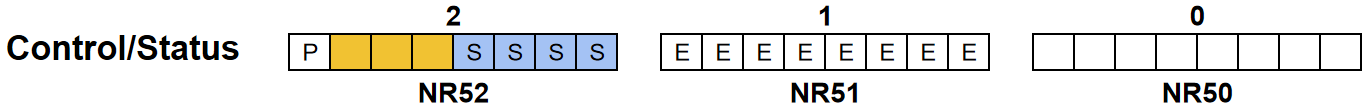
\includegraphics[width=\linewidth]{figures/APU/master_control_apu.png}
    \caption{The registers NR52-NR50, addresses \texttt{0xFF26}-\texttt{0xFF24}, are used for controlling the power and returns the state of all channels. Bits coloured in yellow are write only and will always return 1 if read from. Bits coloured in blue are read only, any data written to this location will be ignored \cite{AudioHardware}.}
    \label{fig:apu_master_control}
\end{figure}

\begin{table}[h]
    \centering
    \begin{tabular}{|c|c|c|}
        \hline
        \textbf{Label} & \textbf{Name} & \textbf{Functionality} \\
        \hline
        P & Power & Enables or disables the entire APU \\
        \hline
        S & State & State of each channel, if 1, the channel is playing \\
        \hline
        L & Left enable & \multirow{2}{*}{\shortstack{Enables or disables left and\\right side for each channel}} \\
        \cline{1-2}
        R & Right enable & \\
        \hline
    \end{tabular}
    \caption{Description of the labels in Figure \ref{fig:apu_master_control}. From \cite{AudioHardware}. Adapted with permission.}
    \label{tab:control_reg_table}
\end{table}

% The registers shown in figure \ref{fig:apu_master_control} displays the registers which controls and shows the power state of all channels. The bit labelled with ``P'' turns on or off the audio hardware and the four bits labelled with ``S'', corresponding to one channel each, is equal to 1 if the channel is playing, and 0 if it does not. The bits labelled with ``E'' also correspond to specific channels and enables or disables the left or right side for each channel. The upper four bits enables or disables the left side, while the lower four bits enables or disables the right side \cite{AudioHardware}.
\newpage
\subsection{Events}
The registers described above trigger events at different frequencies. At what frequency these events should be triggered and exactly what happens at these events is controlled by the registers. Note that all values which are changed with these events are reset when the bit labelled with ``T'' is set \cite{AudioHardware}. The table below summarises the events which occur and at what frequency.
            
\begin{table}[H]
    \centering
    \begin{tabular}{|c|c|c|}
        \hline
        \textbf{Event} & \textbf{Frequency [Hz]} & \textbf{Action} \\
        \hline
        Play sample & \texttt{0x20000}$/(\texttt{0x800} - F)$ & Play next audio sample \\
        \hline
        Play sample (Noise) & \texttt{0x80000}$/ (D * 2 ^ {(S + 1)})$ & Play next audio sample \\
        \hline
        Volume envelope & \texttt{0x40}$/P$ & 
        $V =
        \begin{cases}
            V - 1  & \text{ if A = 0} \\
            V + 1 & \text{ if A = 1}
        \end{cases}$ \\
        \hline
        Length sweep & \texttt{0x100} & Decrease L if length is enabled\\
        \hline
        Frequency sweep (Pulse 1) & \texttt{0x80}$/P$ &
        $F =
        \begin{cases}
            F + F/2^{S}  & \text{ if N = 0} \\
            F - F/2^{S} & \text{ if N = 1}
        \end{cases}$\\
        \hline
    \end{tabular}
    \caption{F, D, S, V, P, L - The value of the bits labelled with ``F'', ``D'', ``S'', ``V'', ``P'', ``L'' respectively, for each channel.}
    \label{tab:frequent_events_apu}
    
\end{table}
      
\subsection{The audio data} \label{sec:theAudioData}
    The pulse wave channels can play a pulse wave with four different waveforms. What waveform to play is specified by the ``duty''-bits, i.e. the bits labelled with ``D'' in Figure \ref{fig:apu_channel_registers}. The resulting waveforms can be seen below in Figure \ref{fig:square_wave_forms}.
        
\begin{figure}[H]
    \centering
    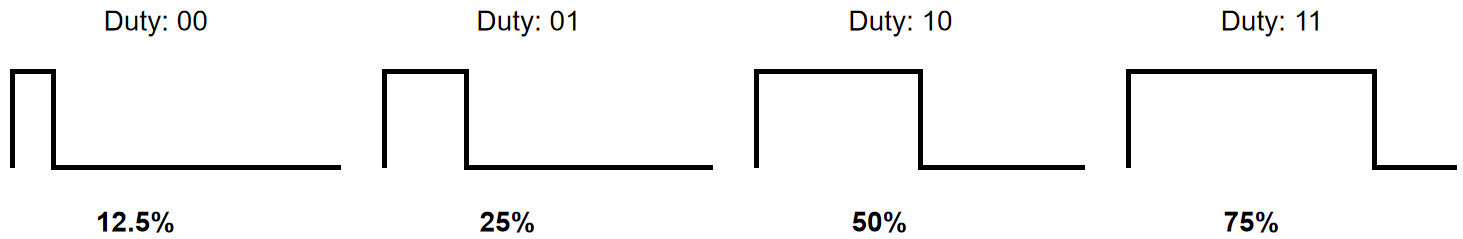
\includegraphics[width=\textwidth]{figures/APU/square_waveforms.png}
    \caption{The four pulse waveforms with their corresponding duties \cite{AudioHardware}. The percentages indicate what amount of the wave is high. Duty ``10'' is   most commonly used.}
    \label{fig:square_wave_forms}
\end{figure}

The waveform of the wave channel can be set to any shape you want by writing to the addresses \texttt{0xFF30} to \texttt{0xFF3F}. Each set of four bits represent one sample which means one waveform consists of 32 samples \cite{AudioHardware}. This approach enables the game developers to create something completely custom made to make their own unique sounds.
\begin{figure}[H]
    \centering
    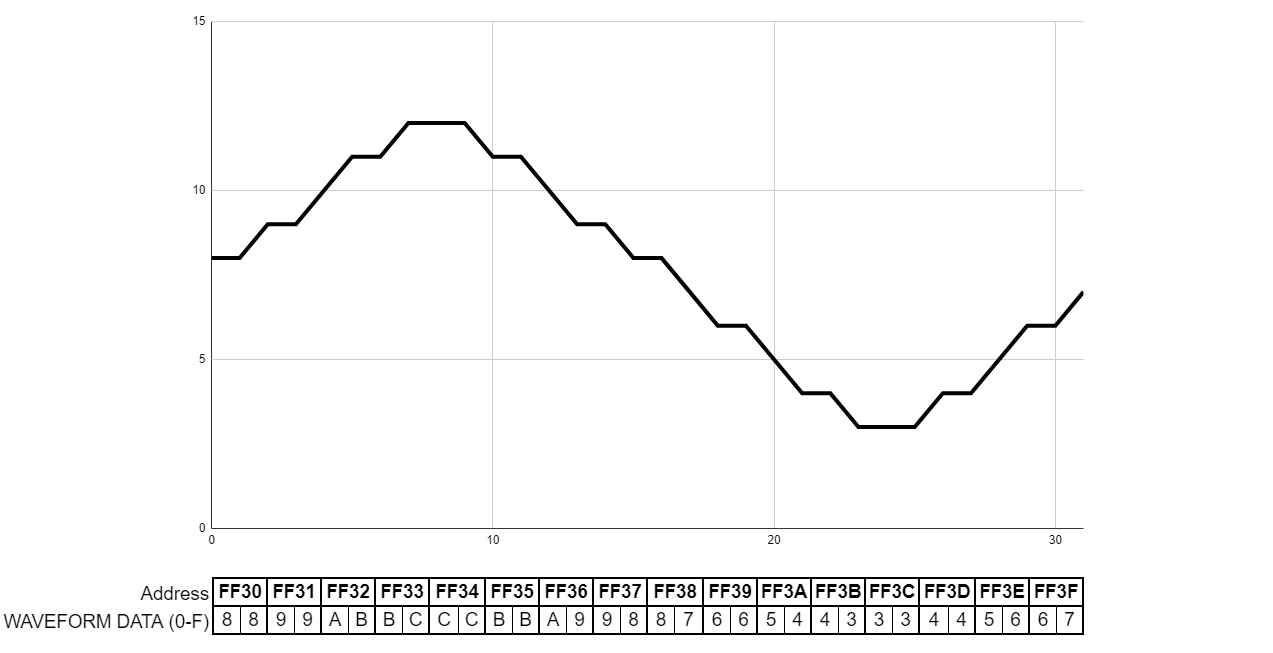
\includegraphics[width=1\textwidth]{figures/APU/apu_custom_waveform.png}
    \caption{A rough representation of how a custom waveform is created through addresses \texttt{0xFF30} to \texttt{0xFF3F}.}
    \label{fig:custom_wave_form}
\end{figure}

The noise channel generates a pseudo-random waveform using a Linear-Feedback Shift Register (LFSR) \cite{apuNoise}. The LFSR is 15 bits long and all bits are set to $1$ in the beginning of the process. Bit 0 in the LFSR determines the output of each sample, if bit 0 is set to one, the output is low, otherwise it is high. To generate a new value of LFSR, the following is calculated where $LFSR(x)$ is the new value, $LFSR(x-1)$ is the old value, $LFSR(x-1)_n$ is the value of bit $n$ in the old value, and $W$ is the value of the bit labelled with ``W'' in Figure \ref{fig:apu_channel_registers} \cite{AudioHardware}.
\begin{equation*}
    LFSR(x) =
    \begin{cases}
        (LFSR(x-1)_0 \oplus LFSR(x-1)_1)*\texttt{0x4000} + LFSR(x-1)/2 & \text{ if W = 0} \\
       (LFSR(x-1)_0 \oplus LFSR(x-1)_1)*\texttt{0x40} + LFSR(x-1)/2 & \text{ if W = 1}
    \end{cases}
\end{equation*}
